\section{Data Collection}
\label{data_collection}

In order to start working, we obviously needed some data. This section presents the three methods we used in order to get samples of acceleration data. The resulting dataset will be analysed (Section \ref{}) and tested in order to find the best way to collect such data on a vehicle.

\subsection{Robot}
Being able to collect our own data is a huge advantage because we can also record metadata that can become handy for better understanding the raw accelerometric data but also for future experiments (for instance, comparing two captors or their placement on the vehicle).\\

It was possible thanks to the acquisition of a brand new radio-controled robot for the Télécom Physique Strasbourg Innov'Lab. This vehicle robot, an Agile-X Scout 2.0, is built for outdoor operations meaning it is perfectly suited to roll on bumps and cracks we had already spotted in the school parking lot.\\

Instead of waiting for our application, we decided to speed-up the process by using an Arduino to collect data. We paired an Arduino Nano with a fairly affordable but reliable IMU: an MPU-6050, which is a common module for DIY drones hobbyists and a micro-SD card module in order to record acceleration data. At the beginning, we also wanted to connect a \textit{Real Time Clock} (RTC) module and a GPS module (respectively a DS1307 and a BN-880) in order to track both time and position but we had to settle back for only acceleration data due to Arduino and I²C bus limitations.\\

After a lot of prototyping and debugging (Figure \ref{bread}), we were finally ready to build a \textit{Printed Circuit Board} (PCB) to conveniently hold the components together, removing any risk of disconnection during data collection. We designed the PCB with Ki-Cad (Figure \ref{pcb_preview}) and quickly made two of them with the school FabLab milling machine (Figure \ref{}).\\

In order to properly mount this little device on the robot, we designed a mounting plate in Solidworks that would acomodate us with many mounting holes for both mount the plate on the robot and mount our devices on the plate. A FabLab manager helped us to laser-cut it in a large piece of acrylic (Figure \ref{robot_1}).\\

\begin{figure}
    \center
    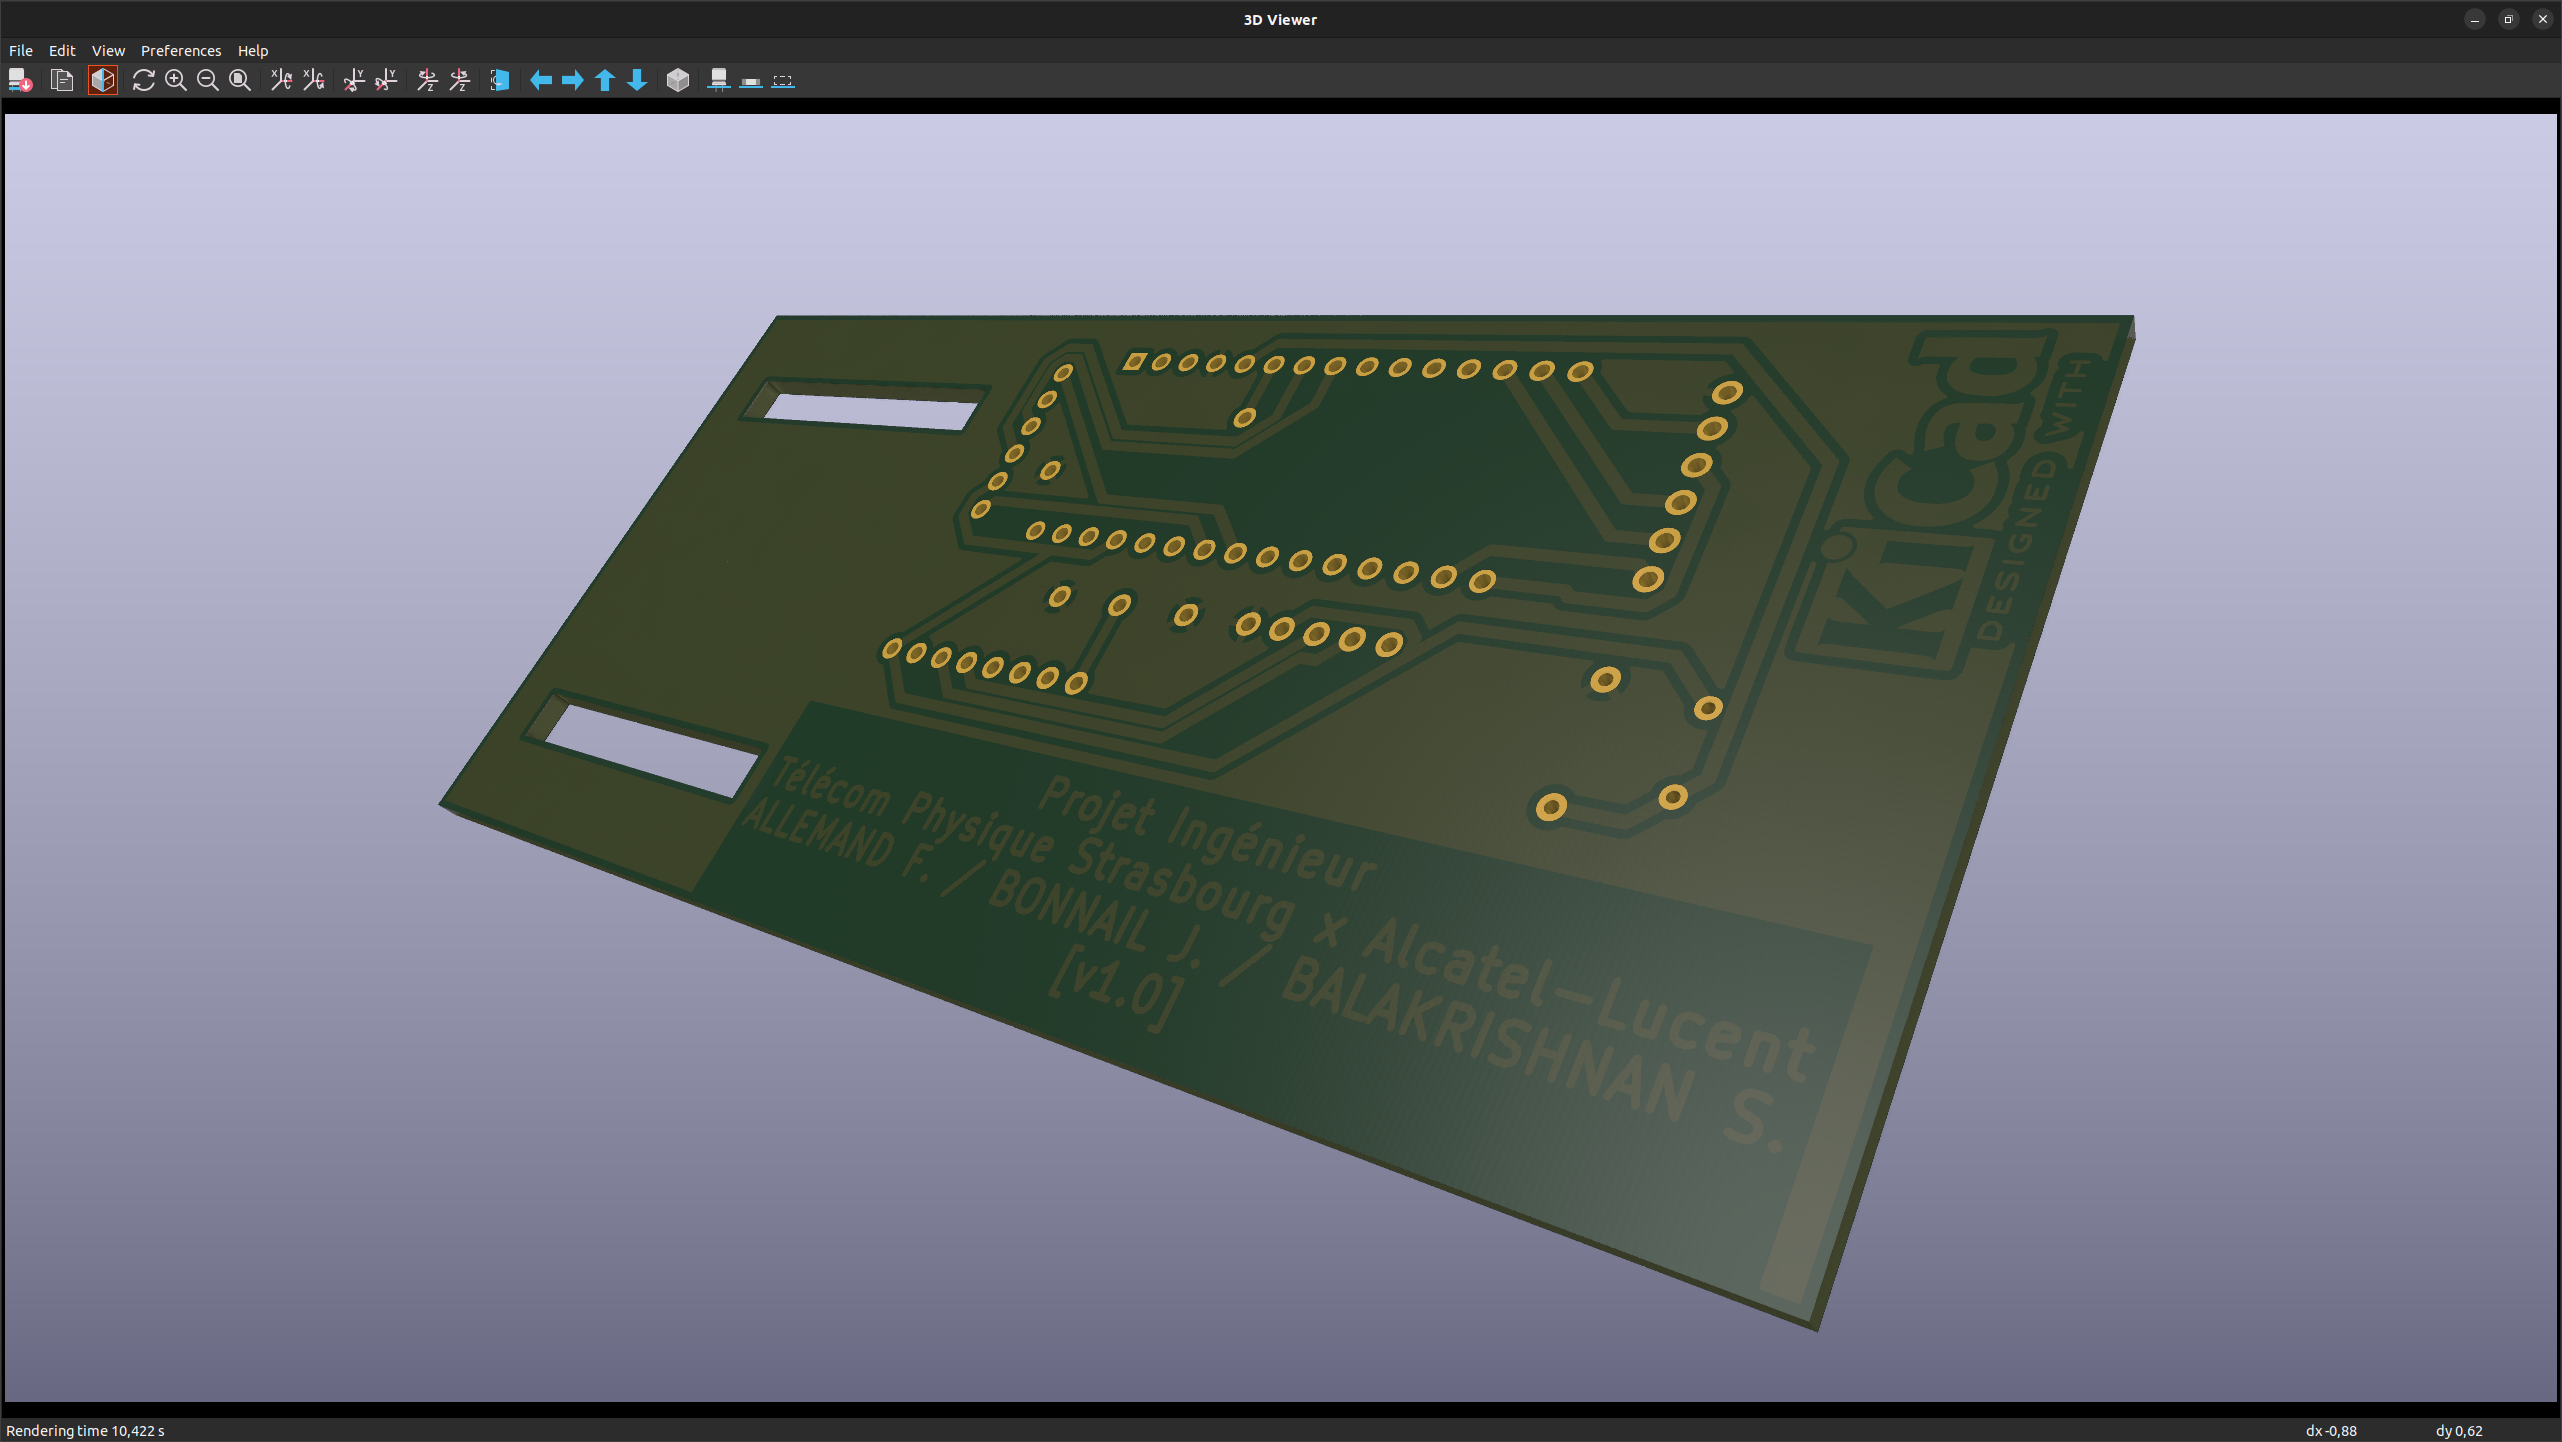
\includegraphics[scale=.12]{img/pcb_preview.png}
    \caption{Preview of the Arduino device PCB}
    \label{pcb_preview}
\end{figure}

\begin{figure}
    \center
    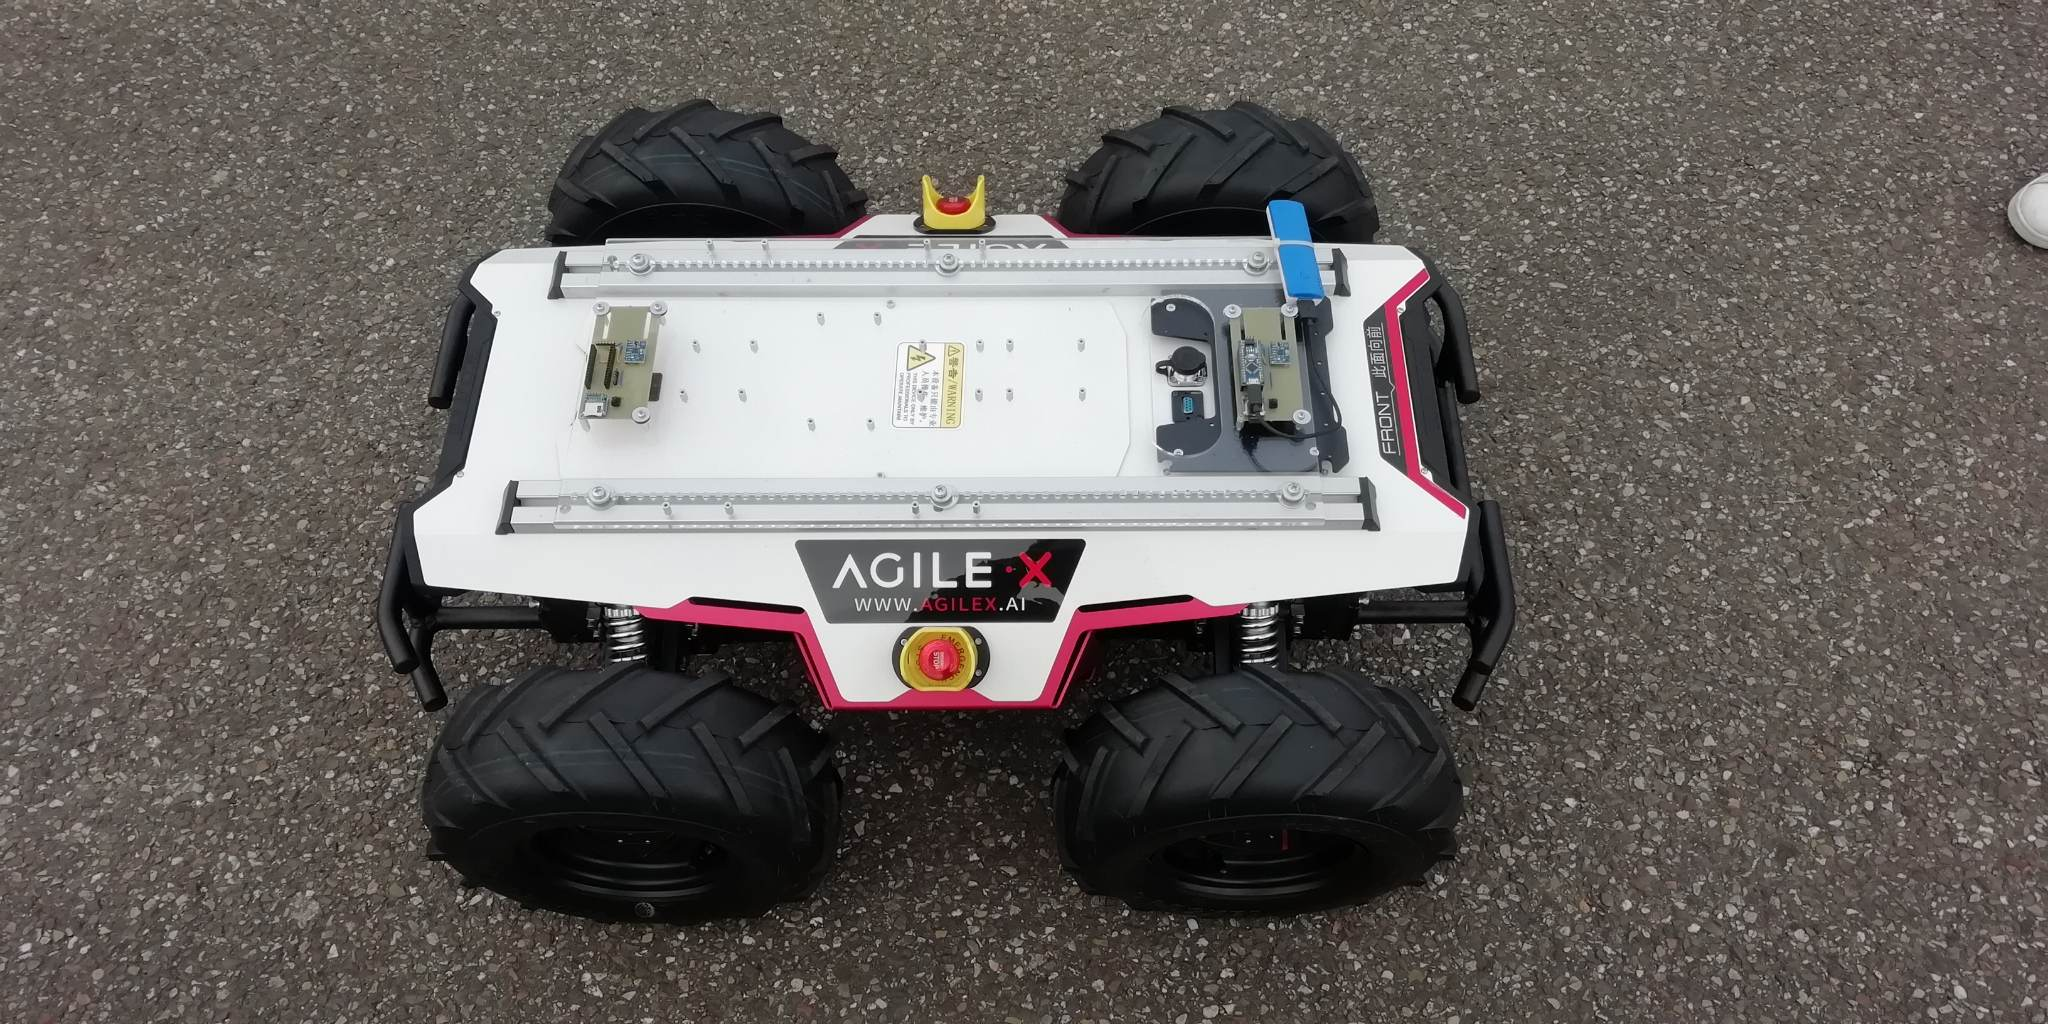
\includegraphics[scale=.15]{img/robot_1.png}
    \caption{Arduino devices mounted on the robot vehicle}
    \label{robot_1}
\end{figure}

\subsection{Car}

\subsection{Online Dataset}

% Data base ?